% TeX'ing this file requires that you have AMS-LaTeX 2.0 installed
% as well as the rest of the prerequisites for REVTeX 4.0
%
% See the REVTeX 4 README file
% It also requires running BibTeX. The commands are as follows:
%
%  1)  latex apssamp.tex
%  2)  bibtex apssamp
%  3)  latex apssamp.tex
%  4)  latex apssamp.tex
%
%\documentclass[prb,showkeys,preprintnumbers,amsmath,amssymb, 11pt]{revtex4}
%\documentclass[preprint,showpacs,showkeys,preprintnumbers,amsmath,amssymb]{revtex4}

% Some other (several out of many) possibilities
%\documentclass[preprint,aps]{revtex4}
%\documentclass[aps, two column, amsmath,amssymb,floatfix]{revtex4}
%\documentclass[showkeys,showpacs,amsmath,amssymb,twocolumn,superscriptaddress,prl]{revtex4-1}% Physical Review B  
\documentclass[aps,prl,reprint,showpacs,floatfix,superscriptaddress]{revtex4-2}

\usepackage{amsmath,amsthm,amssymb}
\usepackage{graphicx}% Include figure files
\usepackage{dcolumn}% Align table columns on decimal point
\usepackage{bm}% bold math
\usepackage{color}
\usepackage{epsfig}
\usepackage{multirow}
\usepackage{mathrsfs}
\usepackage{hyperref}
\usepackage{cleveref}
\usepackage{epstopdf}
\usepackage{subfigure}
\usepackage{autobreak}

%Macros for mathematical notations

\newcommand{\V}[1]{\boldsymbol{#1}} %# vector
\newcommand{\M}[1]{\boldsymbol{#1}} %# matrix
\newcommand{\Set}[1]{\mathbb{#1}} %# set
\newcommand{\D}[1]{\Delta#1} %# \D{t} for time step size
\renewcommand{\d}[1]{\delta#1} %# \d{t} for small increment
\newcommand{\norm}[1]{\left\Vert #1\right\Vert } % norm
\newcommand{\abs}[1]{\left|#1\right|} %abs

\newcommand{\grad}{\M{\nabla}} %gradient
\newcommand{\av}[1]{\left\langle #1\right\rangle } %take average

\newcommand{\sM}[1]{\M{\mathcal{#1}}} %matrix in mathcal font
\newcommand{\dprime}{\prime\prime} % double prime
%\global\long\def\i{\iota}
%\renewcommand{\i}{\iota} %i for imaginary unit
%\renewcommand{\i}{\mathsf i} %i for imaginary unit
\newcommand{\follows}{\quad\Rightarrow\quad} %=>
\newcommand{\eqd}{\overset{d}{=}} %=^d
\newcommand{\spe}[1]{\mathscr{#1}}  %important quantities in mathscr font
\newcommand{\eps}{\epsilon}


\begin{document}
\preprint{Preprint}

\title{Induced Charge Oscillations in Dielectric Confined Quasi-2D Systems}

\author{Xuanzhao Gao}
\email{xz.gao@connect.ust.hk}
\affiliation{Thrust of Advanced Materials, The Hong Kong University of Science and Technology (Guangzhou), Guangdong, China}
\affiliation{Department of Physics, The Hong Kong University of Science and Technology, Hong Kong SAR, China}

\author{Zecheng Gan} \thanks{Corresponding author}
\email{zechenggan@ust.hk}
\affiliation{Thrust of Advanced Materials, The Hong Kong University of Science and Technology (Guangzhou), Guangdong, China}
\affiliation{Department of Mathematics, The Hong Kong University of Science and Technology, Hong Kong SAR, China}

\date{\today}

%%%%% Begin Abstract %%%%%%%%%%%
\begin{abstract}
    We present an analytical solution for the Green's function of dielectric confined quasi-2D systems, which have been challenging to investigate theoretically and with simulations due to difficulties in handling dielectric mismatches. 
    Our solution reveals that under specific confinements, the induced surface charge of an ion exhibits oscillatory behavior, with the wavelength determined by the permittivity and geometry of the system. 
    We have also developed an efficient and accurate algorithm for calculating the electrostatic interaction between mobile ions, facilitating the study of related physical systems using the molecular dynamics algorithm. 
    Our numerical results demonstrate that the substrate permittivity alone can trigger the formation of lattice-like structures of ions due to the oscillatory nature of the induced surface charge. 
    Our findings provide new insights into the behavior of ions in confined geometries and have potential applications in designing new electronic devices.
\end{abstract}

%%%%% end %%%%%%%%%%%

%%%%% AMS/PACs/Keywords %%%%%%%%%%%
%\pacs{no longer needed}

%\keywords{ }
%%%% maketitle %%%%%
\maketitle

%%%% Start %%%%%%

% merge them into one paragragh about quais-2D charged systems
% Among various long-range systems, quasi-2D charged systems are of great importance and have caught much attention recently because of their huge potential in future nanodevices and advanced materials.
\textit{Introduction.}--Quasi-2D systems are defined as systems with a nano-sized longitudinal thickness in the z direction, typically achieved through confinement, which are bulk-like and modeled as periodic in the transverse xy directions. 
These systems exhibit rich new collective behaviors, such as polyelectrolyte adsorption and structure, ion transport, and selectivity, that have garnered much attention. Interestingly, most of these effects are related to the permittivity, specifically the dielectric confinement effect. 
Substrate materials for nanoscale confinement can range from dielectric to metallic, and electromagnetic metamaterials, with permittivities that can take negative values under excitation by electromagnetic waves of specific frequencies, have become increasingly important. 
Significant efforts have been made to develop negative permittivity materials at very low frequencies, and recent work has demonstrated that negative static permittivity can be achieved in a wide range of materials, including metals, quasi-2D crystals, nanoparticles, and polymeric systems.

For electrolytes/polymers near a single dielectric substrate, recent calculations have revealed that the dielectric surface effect can significantly deviate the systems from bulk behaviors, such as ion transport, polymer brush structure, and pattern formation in dipolar films, especially when the permittivity of the substrate is negative.
However, adding a second dielectric substrate to form dielectric confinement in computer simulations is not straightforward. 
While simulation techniques have made significant progress over the past decades, properly treating the dielectric confinement effect with satisfactory accuracy and efficiency remains challenging.

In this letter, we present a novel method for calculating the electrostatic interaction between charged particles in quasi-2D systems under dielectric confinement. 
Our method employs proper renormalization techniques to accurately calculate the electrostatic interaction in metamaterial-confined systems. 
Furthermore, we introduce a lattice summation formula that allows for efficient simulation of charged particles in these systems with spectral convergence.
By applying our method, we investigate the induced surface charge oscillations on substrates under metamaterial confinement. 
Through molecular dynamic (MD) simulations of a prototypical charge- and size-symmetric binary mixture of particles described by the primitive model, we explore the effect of surface polarization on ionic distributions. 
Our results demonstrate that the polarization charge on the surface can induce the system to form lattice-like structures, and the size of the lattice cell can be controlled by tuning the permittivity and thickness of the system. 
This work sheds new light on the complex collective behaviors of charged particles in quasi-2D systems and provides a powerful tool for studying the electrostatic interaction in confined systems.


\begin{figure}[htbp]
	\centering
	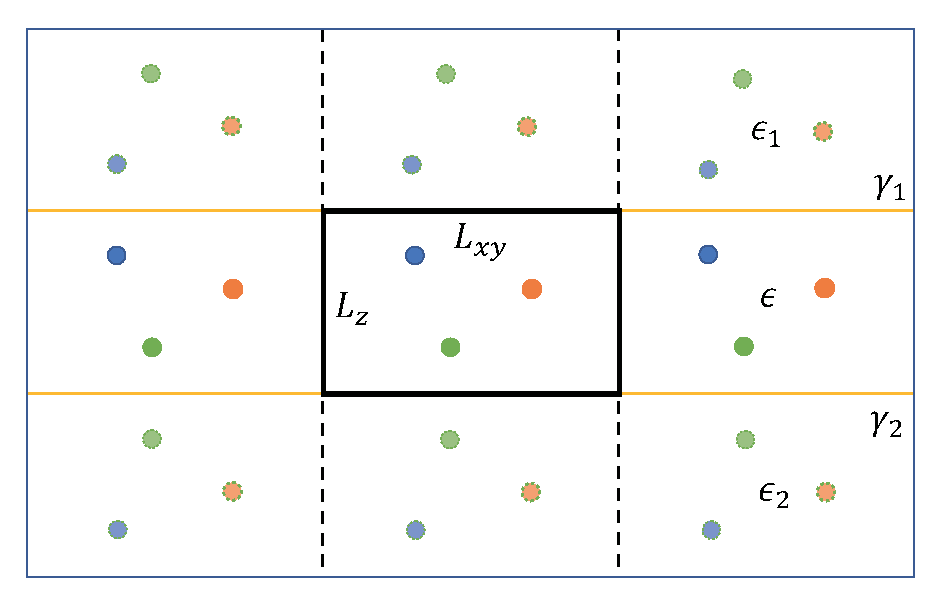
\includegraphics[width=0.45\textwidth]{figs/fig1.pdf}
	\caption{
		This is a schematic depiction of a quasi-2D charged system, illustrating the dielectric confinement effect from the Image Charge Method (ICM) viewpoint. 
        The system consists of a middle layer representing the solvent medium with dielectric permittivity ε, and upper and lower layers representing the substrate with dielectric permittivity ε1 and ε2, respectively. 
        The colored circles surrounded by solid lines represent the real charged particles of the doubly-periodic system, while the ones surrounded by dotted lines represent the image charges reflected by the dielectric interfaces in the z direction.
		\label{fig:ICM}
	}
\end{figure}


% To gain insight into the role of dielectric confinement in quasi-2D systems, we start our discussion with the classic Image Charge Method (ICM). 
% Consider a point charge~$q$ located in a medium with dielectric constant~$\epsilon$ and is near a single planar substrate with dielectric constant~$\epsilon_s$, the polarization potential can be equivalently expressed as the Coulomb potential generated by an image charge located with mirror-symmetry, and magnitude~$q_{\mathrm {img}}=\gamma q$.
% The dimensionless coefficient~$\gamma = (\eps - \eps_s)/(\eps + \eps_s)$ quantifies the strength of polarization, and in the following discussion, we will keep~$\eps = 1$ unchanged when tuning~$\gamma$. 
% Usually,~$\abs{\gamma}\leq 1$ for materials with positive permittivity, but the upper bound can be further lifted for metamaterials because of their stronger polarizability, characterized by negative static permittivity values~\cite{urzhumov2012magnetic, coffey2012magnetic}, so that that~$\gamma$ can be tuned into a much more comprehensive range.

\textit{The model.}--The simulation model comprises a quasi-2D system that is finite in the longitudinal direction and doubly periodic in the transverse direction, with edge lengths of $L_x$, $L_y$, and $L_z$. 
The charged particles are distributed between two dielectric substrates with dielectric permittivity $\epsilon_1$ and $\epsilon_2$, and the system is immersed in a solvent with dielectric permittivity $\epsilon$. 
The strength of polarization is characterized by the dimensionless coefficient reflection rates $\gamma_1$ and $\gamma_2$, which are defined as $(\epsilon-\epsilon_i)/(\epsilon+\epsilon_i)$, where $i=1,2$. 
A multiple reflection process is employed to construct the Green's function of Poisson's equation in the system, resulting in an infinite image charge series, as illustrated in Fig.~\ref{fig:ICM}. 
The image reflection series is convergent when $|\gamma_1\gamma_2|\leq 1$, but it becomes divergent when $|\gamma_1\gamma_2|>1$, and the reflective ICM approach is not applicable. 
The authors have developed a new approach that overcomes this divergence issue by employing a proper renormalization strategy, which enables them to explore the dielectric confinement effect in all possible $\gamma$ regimes, including the scenario of metamaterial substrates with static negative permittivity.


The Green's function $G(\V{r},\V{s})$ for Poisson's equation in a dielectric confined quasi-2D system is given by
\begin{equation}
    -\grad\cdot\left[\eta(\V r) \grad G(\V{r},\V{s})\right] = 4 \pi \d(\V r - \V s )\;,\label{eq:Green4Poisson}
\end{equation}
where $\V{r}$ and $\V{s}$ are the target and source locations, respectively, under the confined geometry. 
Importantly, the relative dielectric function $\eta(\V r) = \eps(\V{r})/\eps$ is piecewise constant, where $\eps(\V{r})$ is the material-specific, spatially varying dielectric constant, defined as in
\begin{equation}
    \eps(\V{r}) = \left\{
    \begin{array}{cc}
        \eps_1,~ & z > L_z \\
        \eps,~ & 0 \leq z \leq L_z \\
        \eps_2,~ & z < 0
    \end{array}
    \right. \;,
\end{equation}
and depicted in Fig.~\ref{fig:ICM}. 
The dielectric interface conditions require the continuity of $G(\V r, \V s)$ and $\epsilon(\V r)\partial_z G(\V r, \V s)$ across $z=0$ and $L_z$, and the free-space boundary condition (FBC) as $z\to\pm\infty$. 
Note that proposing the proper FBC for charges under dielectric confinement requires careful consideration to ensure physical validity, which will be clarified later. 
In the following discussion, we set $\eps=1$ and $\eps_1=\eps_2=\eps'$ so that $\gamma_1=\gamma_2=\gamma$, and by changing $\eps'$, we can vary $\gamma$ from $-10$ to $10$. It is worth noting that the permittivity of VO$_2$ is approximately $-14$ at 350K \cite{kana2016thermally}, and by choosing solvents with permittivity of approximately $11.4$ or $17.1$ (e.g., organic solvents), the proposed $\gamma$ regimes can be experimentally achieved.

\begin{figure}[htbp]
	\centering
	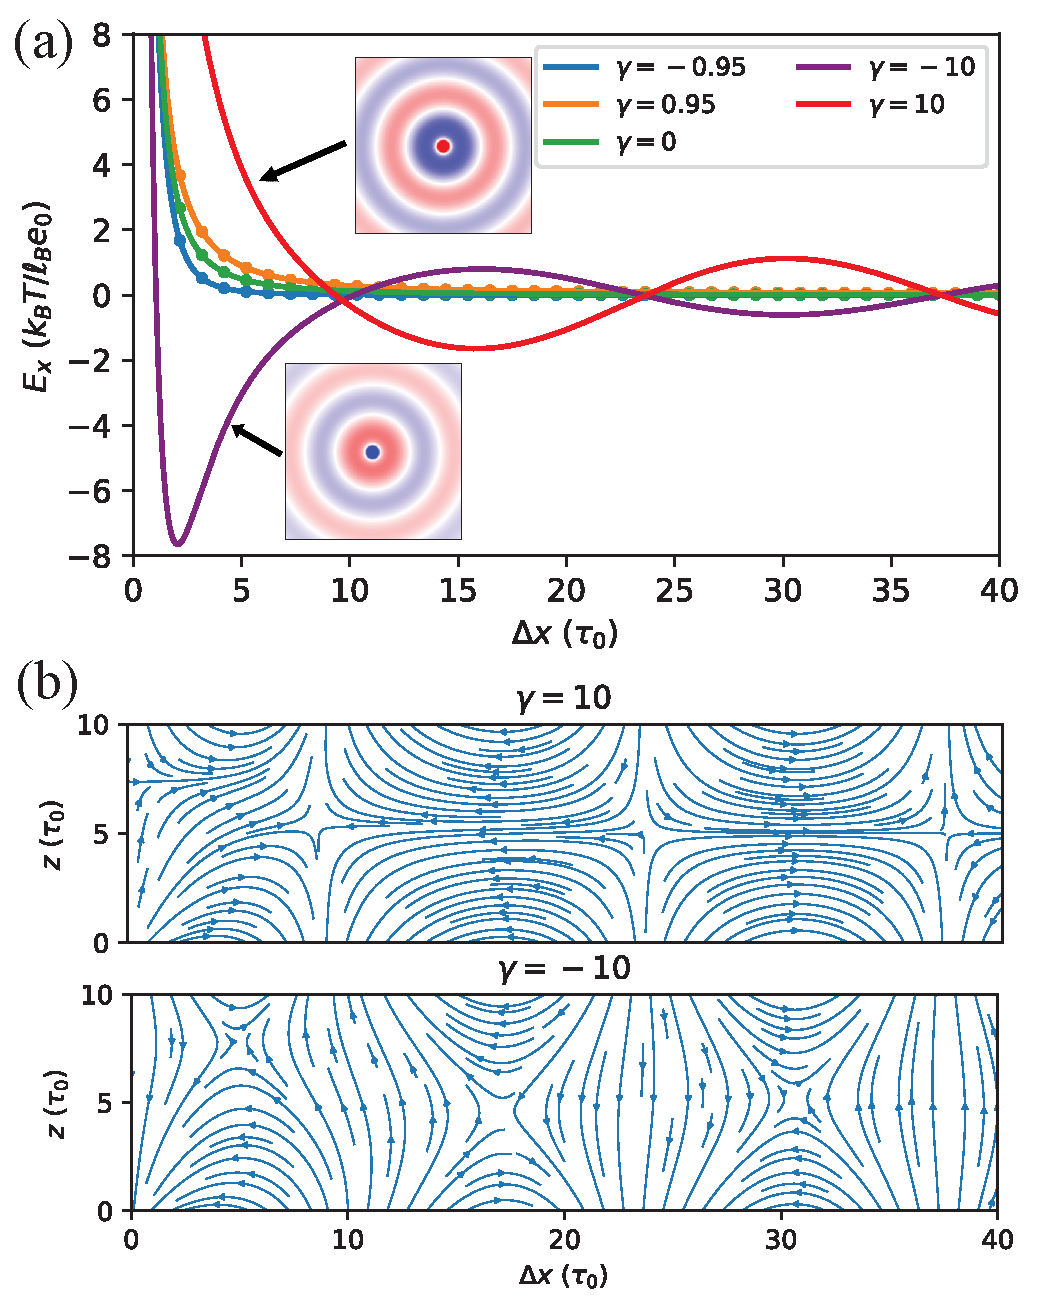
\includegraphics[width=0.45\textwidth]{figs/fig2.pdf}
	\caption{
        Figure (a) displays the electric fields in the $x$ direction generated by a cation with valence $\nu=1$ fixed at $z=\tau_0$ and confined by a pair of dielectric substrates at $z=0$ and $10\tau_0$, where the sub-figures represent the surface charge density on the lower substrates. 
        For the cases where $|\gamma|=10$, the corresponding field lines are plotted in (b).
		\label{fig:force_x}
            }
\end{figure}

% Here the discussion about force between charges should be placed later, after the solution for one point charge is given
\textit{Oscillatory single particle field.}--The dielectric confinement effect is found to be physically attractive even when only one charged particle is present. 
In Fig.\ref{fig:force_x} (a), we plot the electric field in the $x$ direction of a cation with valence $\nu = 1$ at position $(x_0, y_0, \tau_0)$ in a quasi-2D system with a thickness of $10 \tau_0$. 
The confinement is characterized by a reflection rate $\gamma$, and the field is defined as $ - \nu \ell_B \partial_x G(\V r, \V{r_0})$, where $G(\V r, \V{r_0})$ is given in Eq.\eqref{eq:G_pv}, and the coupling parameter $\ell_B = e^2 / (4 \pi \eps_0 \eps k_B T)$ is the Bjerrum length of the solvent with elementary charge $e$, vacuum permittivity $\eps_0$, Boltzmann constant $k_B$, and temperature $T$.
For cases where $\abs{\gamma} < 1$, the Coulomb effect is enhanced or reduced due to polarization on the surface, compared to the $\gamma = 0$ case, as shown by the blue and orange lines in Fig.\ref{fig:force_x} (a), respectively. 
Our method agrees well with ICM, and its results are shown as dots in Fig.\ref{fig:force_x} (a).
However, for cases where $\abs{\gamma} > 1$, the results are highly non-trivial, as shown by the purple and red lines in Fig.~\ref{fig:force_x} (a). 
The short-range interaction behaves as strongly repulsive or attractive when $\gamma = 10$ or $-10$, respectively, which can be seen as an extension of the $\gamma < 1$ cases. Interestingly, the field does not decay to zero but shows oscillatory behavior in the transverse direction, which is different from previous observations.

The polarization charge on the surface at $z=0$, as shown in the sub-figures of Fig.\ref{fig:force_x}(a), explains the non-trivial behavior of the electric field defined by \begin{equation}
    \sigma(\V{r}) = \lim_{z \to 0^+} \nu \ell_B \eps_0  \left( 1 - \frac{\eps}{\eps'} \right) \partial_z G(\V{r}, \V{r_0})\;.
\end{equation}
The field lines generated by the surface charge in the $xOz$ plane are depicted in Fig.\ref{fig:force_x}(b). The oscillatory polarization charge profile leads to this non-trivial electric field behavior. 
At short-range, the strong induced surface charge dominates in both cases, which even reverses the field in the case $\gamma=-10$. 
Surprisingly, the induced charge and field oscillate even at long-range, which is caused by the strong polarization and further enhancement by the bi-surface reflection. 
The oscillatory field reported here has a similar structure to that of a surface plasmonic resonance wave, but a different physical origin. 
Here, the oscillation is due to the reflected polarization enhanced by the dielectric confinements characterized by parameters $\gamma_1$, $\gamma_2$, and $L_z$. 
Particularly, we find that the confinement induced resonance wave number is given by 
\begin{equation}\label{eq:k0}
    k_0 = \frac{\ln{\gamma_1 \gamma_2}}{2 L_z}\;,
\end{equation}
and the \emph{wavelength} $\lambda$ of the oscillation, defined as two times the distance between nearby zeros, satisfies
\begin{equation}\label{eq:wavelength}
    \lambda \cdot k_0 \sim 2 \pi \;.
\end{equation} 
It is numerically validated that Eq.\eqref{eq:wavelength} is highly robust under different choices of $\V{r}$, $\V{r}_0$, $\gamma$, or $L_z$, as shown in Fig.\ref{fig:k_wavelegth}, and the results will be further justified theoretically.
Interestingly, one can accurately predict and control the oscillation fields by adjusting $k_0$. Eq.\eqref{eq:k0} indicates that the oscillation will be weakened as $L_z$ is increased and becomes non-oscillatory when $\gamma_1\gamma_2<1$.

\begin{figure}[htbp]
    \centering
    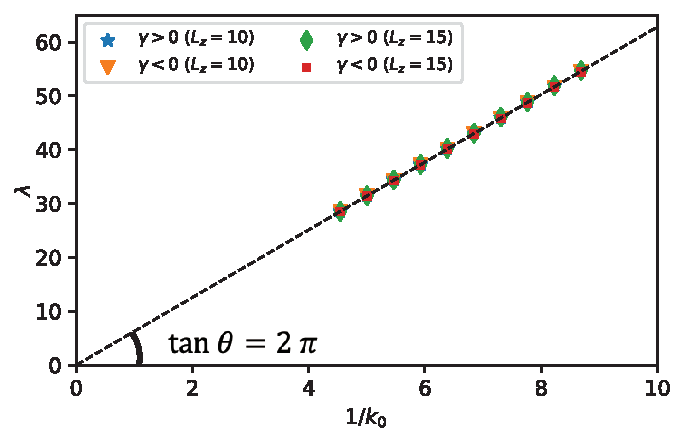
\includegraphics[width=0.45\textwidth]{SIfig/k_wavelegth.pdf}
    \caption{
        Numerical results for relation between~$k_0$ and~$\lambda$.
        The system parameters, $\gamma$ and~$L_z$, are changed to tune~$k_0$.
        For each point in the figure, we calculated the interaction between a pair of particles with randomly generated position in~$z$ as a function of~$\D \rho$.
        Then the average distance between zero points of~$E_x$ is taken as~$\lambda / 2$.
    }
    \label{fig:k_wavelegth}
\end{figure}

To solve the Green's function problem in Eq.\eqref{eq:Green4Poisson}, we can apply plane wave expansion on both sides of the equation, which leads to 
\begin{equation}\label{eq:G_point_charge}
    \begin{split}
        G(\V{r},\V{s}) & = - \frac{1}{\pi} \iint_{\mathbb{R}^2} g(k, z, z_s) e^{-i \V{k} \cdot \Delta \V{\rho}} \text{d} k_x \text{d} k_y \\
        & = - \int_{0}^{+\infty} 2 g(k, z, z_s) J_0(k \Delta \rho) k \text{d}k\;,
    \end{split}
\end{equation}
where $\V{k} = (k_x, k_y)$ and $\Delta \V{\rho} = (x - x_s, y - y_s)$.
When $k>0$, $g(k, z, z_s)$ can be expressed as 
\begin{equation}\label{eq:g_solution}
    g(k, z, z_s) = \frac{1}{2k} \frac{1}{\gamma_1 \gamma_2 \exp{(-2 k L_z)} - 1} \sum_{i = 1}^{4} \Gamma_l \text{e}^{-k a_l}\;,
\end{equation}
where $\Gamma_l = \left[1,\gamma_1,\gamma_2,\gamma_1 \gamma_2 \right]$ and $a_l = [\abs{z - z_s},~z + z_s,~2L_z - (z + z_s),2L_z - \abs{z - z_s}] \in [0, 2L_z]$.
When $k=0$, the solution is given by 
\begin{equation}\label{eq:g_k=0}
    g(k = 0, z, z_s) = - \frac{\abs{z - z_s}}{2}\;.
\end{equation}
Physically, Eq.\eqref{eq:g_k=0} implies that when $k=0$, the confined source charge acts as a uniformly charged plate.

Although the Green's function~$g(k, z, z_s)$ is analytically solvable, the integral in Eq.\eqref{eq:g_solution} diverges for cases where$\gamma_1 \gamma_2 > 1$ because~$g(k, z, z_s)$ diverges at~$k=k_0$, as given in Eq.~\eqref{eq:k0}. 
Therefore, the integral must be renormalized.
Notably, as~$k$ approaches~$k_0$, the divergent factor has the property given in 
\begin{equation}
    \frac{1}{\gamma_1 \gamma_2 \exp{(-2 k L_z)} - 1} \to \frac{1}{2 L_z (k_0 - k)}\;,
\end{equation}
indicating that~$k_0$ is a first-order pole, and the Cauchy principal value exists.
Therefore, for cases where~$\gamma_1 \gamma_2 > 1$, the Green's function is given by 
\begin{equation}\label{eq:G_pv}
    G(\V{r}, \V{s}) = - \text{p.v.} \left[ \int_{0}^{+\infty} 2 g(k, z, z_s) J_0(k \Delta \rho) k \text{d}k \right]  \;,
\end{equation}
and can be calculated numerically.
Eq.\eqref{eq:G_pv} may provide an explanation for the relationship in Eq.\eqref{eq:wavelength}.
All terms in Eq.\eqref{eq:G_pv} can be simplified, as shown in 
\begin{equation}
    I_o = \int_0^{\infty} \frac{J_0(k \D \rho) \text{e}^{-ka}}{\exp{\left( 2 L_z (k_0 - k) \right)} - 1} \text{d}k\;,
\end{equation}
where$\Delta \rho$,$k_0$, and$a$ are all positive constants. 
We find that the oscillation in~$I_o$ can be further transformed, as given by  
\begin{equation}
    I_{o} = \frac{e^{-k_0 a}}{2L_z} \int_0^{\infty} \frac{J_0(k^\prime)}{k_0 - k^\prime} \text{d}k^\prime + f(k_0, \D \rho, a)
\end{equation}
where~$k' = k \Delta \rho$, and~$f(k_0, \Delta \rho, a)$ is a non-oscillatory analytic function that contributes less to~$I_o$. 
Details are shown in the supplementary information (SI).
The first integral can be regarded as a function of~$k_0 \Delta \rho$, labeled as~$I_m(k_0 \Delta \rho)$, which is independent of other parameters and is general for any given parameters. 
Numerical results show that the distance between the zero points of~$I_m(k_0 \Delta \rho)$ converges rapidly to~$\pi$, which leads to the near-periodic property of the field and the relationship given by Eq.~\eqref{eq:wavelength}.

\textit{Collective behaviors.}--To study how the oscillation affects the phase behavior of quasi-2D charged systems, we developed a molecular dynamics (MD) algorithm based on the Ewald splitting method, as described in detail in the SI.
We considered a prototypical quasi-2D charged system, consisting of a binary mixture of charged particles described by the primitive model.
The system contains $N/2$ cations and $N/2$ anions, each with the same diameter $\tau_0$ and valence $\pm 1$, resulting in overall charge neutrality.
Assuming that the $i$-th particle is located at $\V{r_i}$ and carries a charge of $q_i$, the Hamiltonian of the system is given by
\begin{equation}
    \mathcal H = \frac{1}{2} \sum_{i,j=1}^{N}{}^\prime q_i q_j \ell_B G(\V r_i, \V r_j) + U_{\mathrm{LJ}}\;,\label{eq:Hamiltonian}
 \end{equation}
where $\sum_{i,j}{}^\prime$ indicates that when $i=j$, $G(\V r, \V r)$ is the self-interaction, and $U_{\mathrm{LJ}}$ is the shift-truncated Lennard-Jones (LJ) potential energy modeling the excluded-volume interactions.
While the present model does not include other interactions that may be relevant in experimental realizations, it allows us to isolate the dielectric confinement effect.
Similar setups have been investigated in recent studies (Refs. [XX, YY]).

In all Molecular Dynamics (MD) simulations, we fix the box size in the $xy$ plane to be $180\tau_0\times 180\tau_0$ in order to ignore boundary effects in the central area. We tune the values of $L_z$ and $\gamma$ to control the value of $k_0$. The Bjerrum length for the solvent medium is set to $\ell_{\mathrm B} = 3.5 \tau_0$. The temporal integration is performed using the Velocity-Verlet algorithm provided by LAMMPS, and the temperature is controlled via Anderson thermostat with a stochastic collision frequency of $\omega = 0.1$.

\begin{figure}
	\centering
	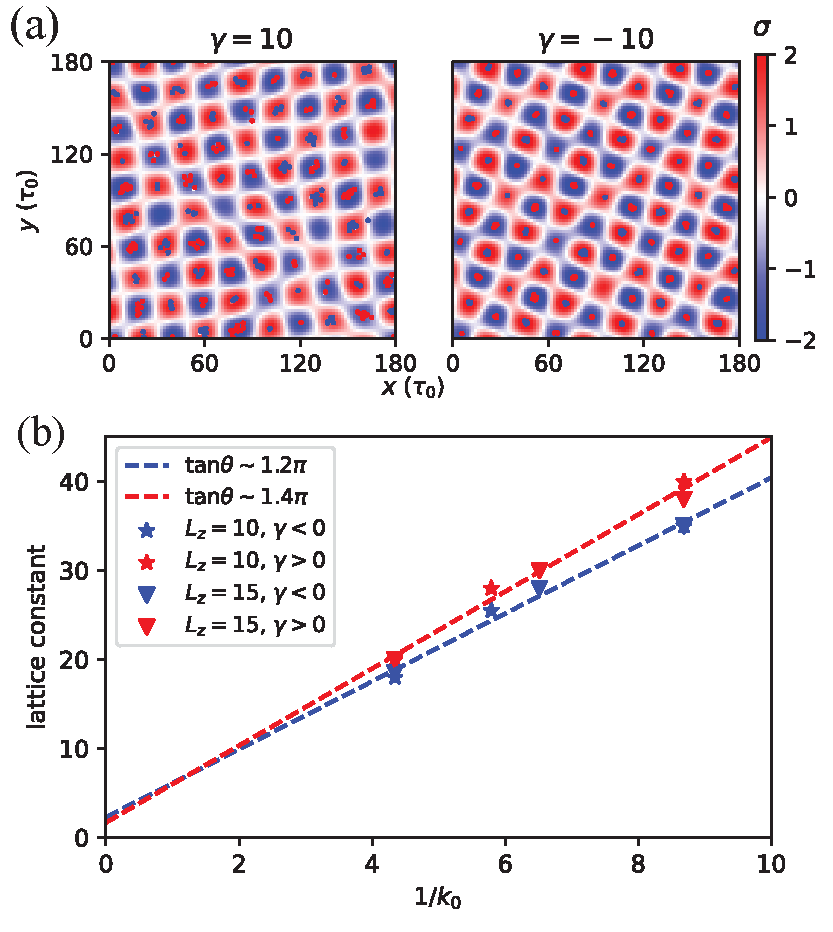
\includegraphics[width=0.45\textwidth]{figs/fig3.pdf}
	\caption{\label{fig:MD} 
        The figure illustrates the charge distribution near the lower substrate and the surface charge density for cases where $\gamma = \pm 10$ and $L_z = 10$ (panel a).
        The positive and negative charges are depicted in red and blue, respectively. 
        Additionally, panel (b) shows the relation between the lattice constant and system parameters. 
        The sampling points are marked with dots, and the dashed lines represent the fitting results.
	}
\end{figure}

Interestingly, we observed the formation of periodic structures near the substrates in both cases where $\gamma > 1$ and $\gamma < -1$ in the transverse direction, as depicted in Fig.\ref{fig:MD}(a). 
In the vertical direction, the ions are distributed near the substrates and are symmetrically or anti-symmetrically paired with another cluster on the opposite side. 
The clusters' structures are different, as the ions are closely packed when $\gamma < -1$ and form an ion liquid when $\gamma > 1$ due to the attractive and repulsive interactions between the charges, respectively, as illustrated in Fig.\ref{fig:force_x}(a).
We attribute the formation of the lattice to the oscillation field induced by a single particle, as depicted in Fig.~\ref{fig:force_x}(a). The field motivates particles to self-organize and enhances the overall induced charge landscape into a "checkerboard" structure with potential wells confining the charges within.

The formed lattice structure is robust and can be controlled via $k_0$, as shown in Fig.~\ref{fig:MD}(b). 
The lattice constant of the system is proportional to $k_0^{-1}$ under different values of $L_z$ and $\gamma$. This mechanism enables us to modulate the collective structure of dielectric confined charged systems.
Moreover, we observed that the slopes are slightly different, $1.2\pi$ and $1.4\pi$, for $\gamma < 0$ cases and $\gamma > 0$ cases, respectively, proportional to the distance between the nearest neighbors. 
These values are close to the second zero point of surface charge excited by a point charge near the surface.

\textit{Conclusions.}--In conclusion, we have demonstrated that polarizable substrates with negative permittivity can induce oscillations in the electric field of a point charge in a dielectric confined quasi-2D system. By utilizing a newly developed lattice summation method, we observed lattice formation in the system due to the collective self-organization of ions under the influence of the oscillatory field, which can be controlled by adjusting the resonance frequency~$k_0$. Our approach provides an efficient and accurate simulation tool for a broad range of quasi-2D systems, with potential applications in future nanotechnology. Further investigations on the phase behavior of dielectric confined quasi-2D charged systems are warranted. Moreover, an open source implementation of our method in LAMMPS~\cite{LAMMPS} is planned for future development.

\end{document}
